%# -*- coding: utf-8-unix -*-
% !TEX program = xelatex
% !TEX root = ../thesis.tex
% !TEX encoding = UTF-8 Unicode
%%==================================================
%% chapter01.tex for SJTU Master Thesis
%%==================================================

%\bibliographystyle{sjtu2}%[此处用于每章都生产参考文献]
\chapter{Introduction}
\label{chap1}
\section{Introduction}
People have their own opinions, and sometimes they change their opinions in response to others who have views on those issues. Their opinions are reflected in the leaders to make laws and make necessary decisions. These phenomena can be found in some cases, such as voting, legislation, and the adoption of new policies. It is widely recognized that both opinion formation and decision-making formation have mutual interaction as interconnected networks\parencite{mikko2014, danziger2019, newman2010, boccaletti2014, domenico2013, tomasini2015, namkhanhvu2017}. Sometimes, opinion formation can be opposed to decision-making formation. These situations often give rise to social conflicts and confusion. In order to figure out these social conflicts, it is necessary to understand and analyze the competition of interconnected networks. So far, physics and computer science have researched these social conflicts by modeling and analyzing complex systems\parencite{fangwu2004, zuev2012, laguna2004, masuda2014}. The researches include opinion dynamics\parencite{amato2017, haibo2017, amato2017, quattrociocchi2014}, voter model\parencite{redner2005, casey2009}, game theory\parencite{smyrnakis2019}, and many more\parencite{bianconi2018}. 
Competition of interconnected networks has been researched in various ways. These networks can be applied to the propagation of computer viruses\parencite{serazzi2003}, information\parencite{hua2014}, opinions\parencite{alvarez2016, gomez2015,diep2017,rocca2014, velasquez2018}, memes\parencite{massad2013}, infections\parencite{shenyu2018, zhou2018}, and rumors\parencite{liu2018}. Opinion dynamics on interconnected networks have been investigated with various network models such as \textit{Abrams-Strogatz(AS)} model\parencite{abrams2003,vazquez2010} and $M$ model\parencite{rocca2014}.  Based on the previous research, this work studies the main features of competition in two-layer networks by changing network structures, changing the updating rules, and selecting the key nodes. It is proven and analyzed that these different conditions cause different results.
\begin{figure}[!htb]
	\centering
	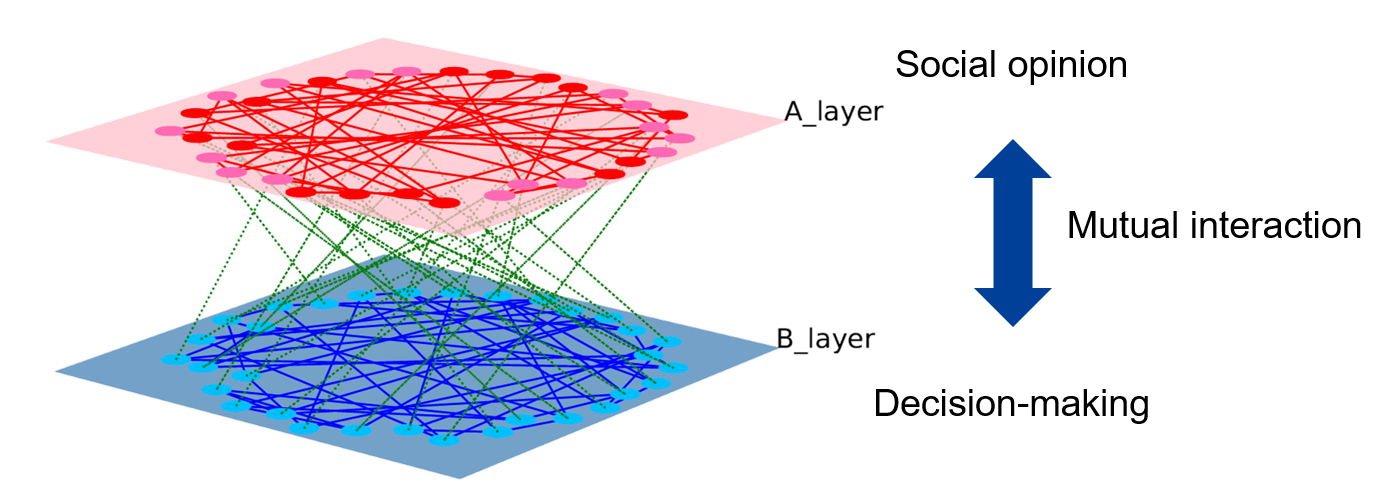
\includegraphics[width=\hsize]{chap1_topic.png}
	\caption{The example of competition on a two-layer network}
	\label{chap1_topic}
\end{figure}

\section{Competition on interconnected networks}
In this research, we focus on the competition on a two-layer network or an interconnected network. If compared with a single-layer network, the interconnected network has two dynamics, two parameters, and includes internal edges and external edges, as shown in Fig.~\ref{chap1_singlemulti}. Therefore, the interconnected network interaction is more complex than single-layer network interaction.

\begin{figure}[!htb]
	\centering
	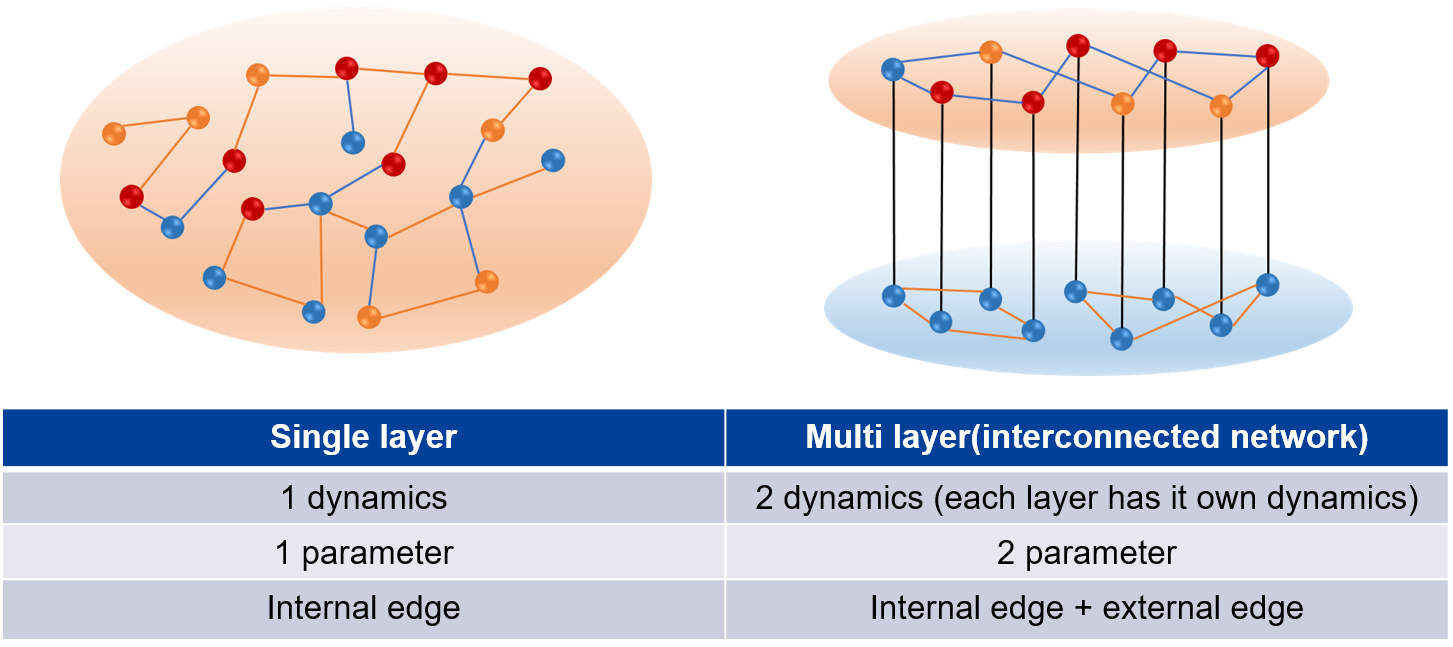
\includegraphics[width=\hsize]{chap1_singlemulti.png}
	\caption{Comparison between a single-layer network and a two-layer network}
	\label{chap1_singlemulti}
\end{figure}

In order to make a two-layer network under competition, each layer consists of different dynamics and parameters. Network dynamics are based on previous research, such as \parencite{alvarez2016}. The top layer has the function of social opinion and its dynamics. Some opinion models provide a social mechanism through the compromise process\parencite{naim2003}. Other opinion models represent the persuasive process\parencite{chau2014}. In this research, the social opinion layer is affected by the opinion dynamics, which are also known as M-model\parencite{rocca2014}, which includes compromise function and persuasion function. The bottom layer has the function of decision-making and its dynamics. The dynamics of the decision-making layer is the language competition dynamics that are also called as the \textit{Abrams-Strogatz} model\parencite{abrams2003, vazquez2010, patriarca2012}. This model is useful to decide only one opinion from two opinions. In order to make the competition condition of these two layers, the initial states of the two layers are assumed to be in opposite states, that the social opinion layer has all positive states, and the decision-making layer has all negative states\parencite{alvarez2016}.

So far, main researchers have focused on what factors make a consensus or dissent(coexistence), which have shown that the system can make positive consensus, negative consensus, or coexistence under a specific range of parameters, such as volatility, reinforcement, strength, and prestige\parencite{alvarez2016}. Moreover, the interconnected competition of the social network has been researched by finding the threshold or critical point for consensus\parencite{alvarez2016, gomez2015, diep2017}. Also, it has been shown that the thresholds make the transition of states, and they can explain and analyze the social phenomena in the real world, such as the legislation, election, and social conflicts\parencite{alvarez2016, gomez2015, amato2017, diep2017}.

In \parencite{gomez2015}, it is shown that the transition from localized to mixed status occurs through a cascade from poorly connected nodes in the layers to the highly connected ones, and the external degree is critical to change the state of the network. Besides, the main features, such as transition and cascade, found in Monte Carlo simulation, are precisely characterized by the mean-field theory and magnetization\parencite{alvarez2016, diep2017, amato2017, gomez2015} .

Based on all this previous research, the competitions of interconnected networks are analyzed by three main topics, such as network structures, updating rules, and selection of key nodes. Theoretically, the previous models have already been proven by using the mean-field theory and magnetization. In this thesis, the models will be analyzed by using computer simulations because applied dynamics are switched according to the state of nodes. In these models, practical mathematical tools cannot be applied\parencite{nicolas2017, rainer2002}. Therefore, computer simulations will be mainly implemented. Before simulations, backgrounds for three topics are explained as follows. 

\begin{figure}[!htb]
	\centering
	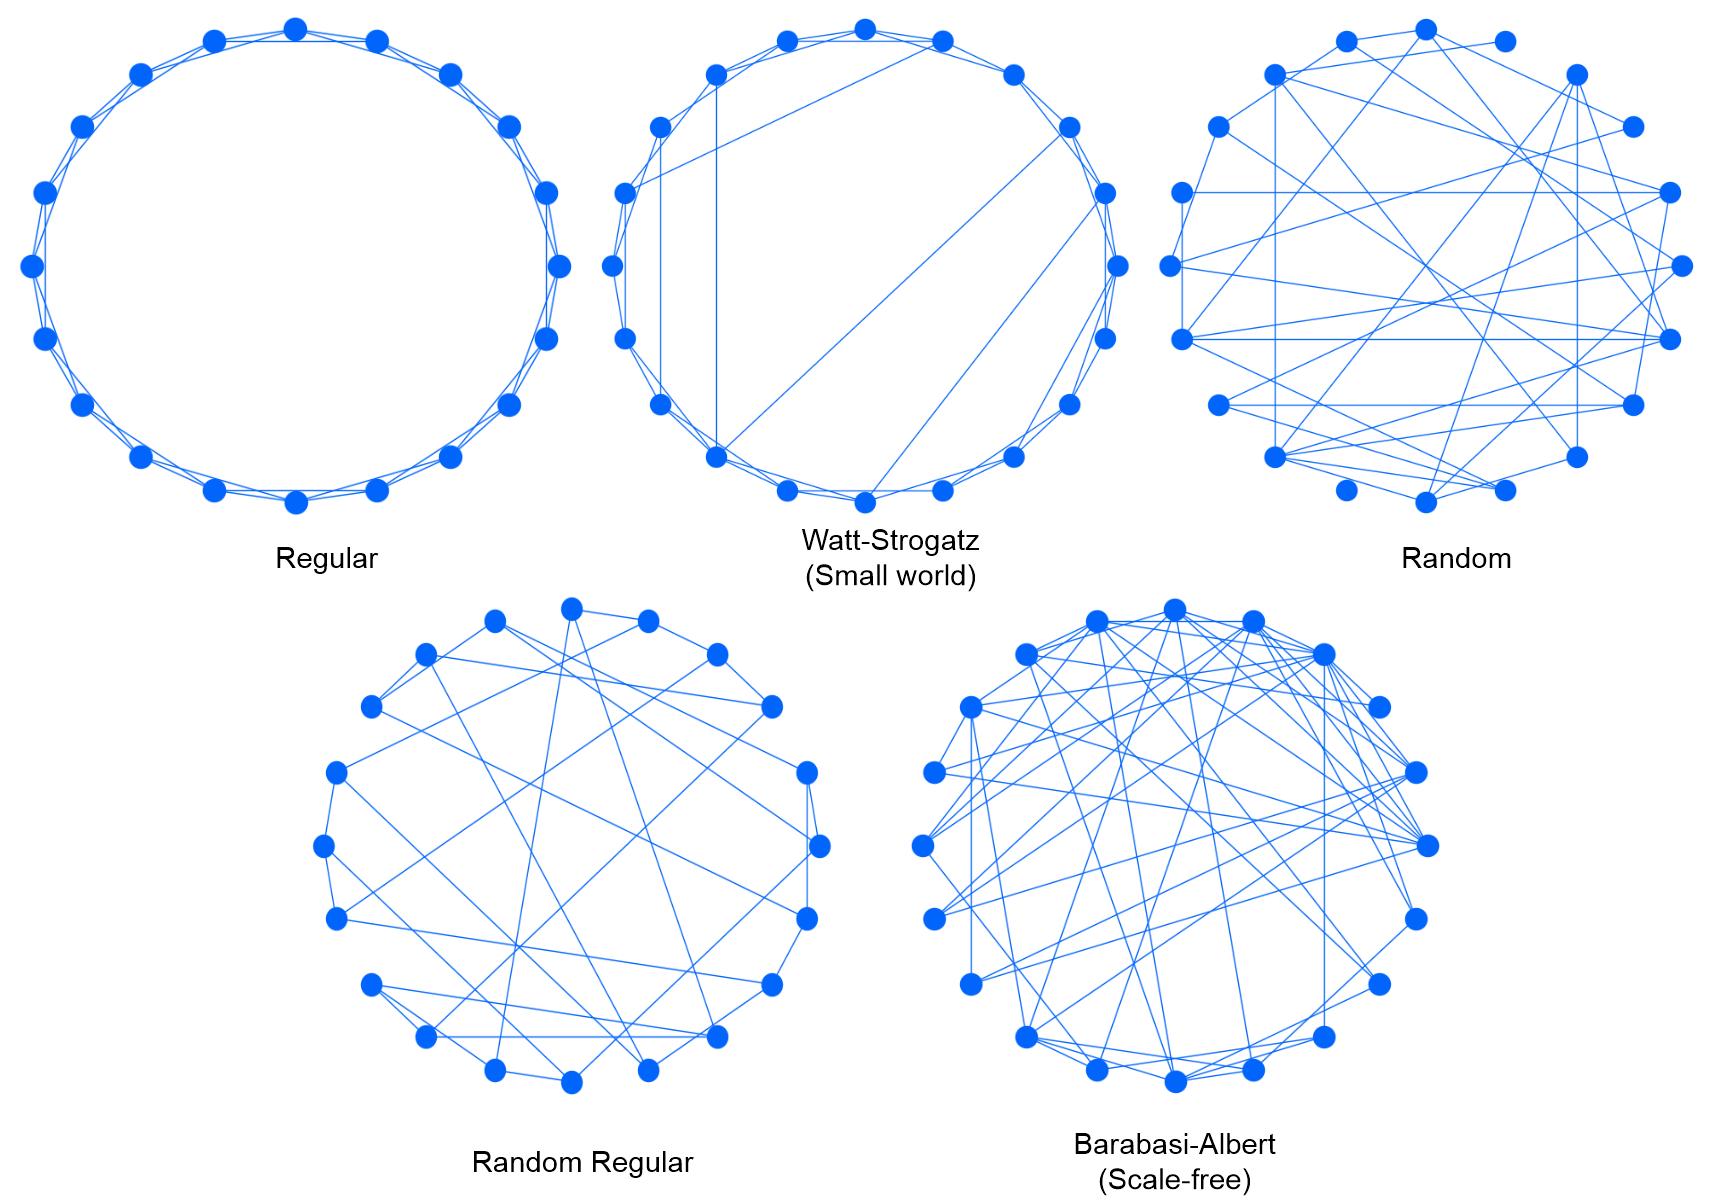
\includegraphics[width=\hsize]{chap1_network_type.png}
	\caption{Various structures of the network}
	\label{chap1_network_type}
\end{figure}

First, network structures are investigated. Networks can be largely divided into a regular network, a random network\parencite{erdos1960}, a small-world network\parencite{watts1998}, a scale-free network\parencite{barabasi2011}, and others. Fig.~\ref{chap1_network_type} shows the structures of various networks. A regular network has a lattice structure, and each node has the same number of links. A random network is made up of edges such that two nodes are connected with probability $p$ in the systems with $K$ nodes. A small-world network is a network type in which most nodes are not neighbors of each other, but most nodes can reach all other nodes through a small number of links. A small-world network can be made by eliminating the edges with probability $p$ and connecting two random nodes that are not connected in a regular network. A small-world network has all characteristics of a regular network and random network. A scale-free network has a model such that the distribution of edges follows power function. Examples of a scale-free network are the World Wide Web (WWW), the Internet, movie star networks, protein interactions, metabolism, and so on. There are several ways to create a scale-free network. Among them, the most typical way is the \textit{Barabasi-Albert} model. The \textit{Barabasi-Albert} model is growing networks in which nodes continue to be added, and connections between nodes have a preferential attachment. The process of creating this model repeats the following two processes: First, add one node with a constant number of edges to the system. Second, edges of the added nodes are connected in proportion to the edge number of the pre-existing nodes. In this work, two types of general networks are applied, such as a random regular(RR) network and \textit{Barabasi-Albert}(BA) network. 

Second, dynamics orders and updating rules are also studied. For further understanding of the competition on a two-layer network, it is crucial to investigate the interaction between nodes or layers. Methods of interaction between nodes are various. However, related to time, the types of interactions can be divided into two categories, such as simultaneous interaction, and sequential interaction\parencite{sirbu2017}. In economics and social networks, it has been proven that there exist different results between simultaneous and sequential interaction\parencite{hoffman2011, dietrich2004}. In \parencite{hoffman2011}, it was researched how experimental subjects update induced prior information when receiving two information signals simultaneously or receiving the same signals sequentially. As the experimental results, the simultaneous method is very different from the sequential method, and under sequential information, the subject’s mean estimates of the two methods(good news preceding bad news or vice versa) are also significantly different from each other. In conclusion, both the sequencing of process and the order of information matters. Moreover, in \parencite{dietrich2004}, the usual random sequential updating rule is displaced by the simultaneous updating rule on the \textit{Sznajd} model. It is found out that this change makes a complete consensus much more difficult. The reason is analyzed as some agents with the simultaneous updating rule receive conflicting messages from different neighbor pairs and thus refuse to change their opinion. In this work, both simultaneous and sequential updating rules are applied to layers, nodes, and links.

Third, network centralities are researched to select key nodes on a two-layer network. Network centrality means the index to measure how close each node is to the center of a network. That answers the question, "What characterizes an important node?". The theory of network centrality was first introduced in the field of social network analysis\parencite{freeman1979}. After that, it has expanded to various areas where the concept of the network is related and has been used to identify which nodes are important in the network. So far, various criteria for assessing network centrality have been presented. Generally, well-known network centralities include degree centrality, betweenness centrality, closeness centrality, eigenvector centrality, and Pagerank\parencite{koschutzki2008, francisco2018, bianconi2018}. Degree centrality is the simplest but the most reliable concept. It is defined as the number of interacting neighbor nodes (or edges).  Betweenness centrality is the notion of using the shortest path between two nodes on a network. It is explained as the concept to define two different node sets on the network (set $1$, $2$) and quantify how often each node appears on the shortest path for all combinations of nodes in set $1$ and set $2$. Closeness centrality is derived from that the shorter the path that one node reaches all the other nodes is, the more influential the node is. Eigenvector centrality is the concept that the more a node is connected with critical nodes, the more critical it is. Pagerank measures the convergent value by repeating the process of propagating each node's influence on the other nodes.
So far, many researchers have tried to select critical nodes in a social network\parencite{eom2015, white2003, mesgari2015, hwang1981, huang2014}. Based on a node centrality, some algorithms for identifying key nodes has been found out. In \parencite{mesgari2015, huang2014}, it has been found out that optimally combining multiple measures of nodal importance may provide a robust tool for identifying key nodes of interest, particularly in large graphs. Here, based on previous research, we select the key nodes by using a single node centrality and combined node centrality.

In this work, for single indicator methods to select key nodes, network centralities will be applied, such as Pagerank, degree, eigenvector, betweenness, and closeness. As multiple indicator methods recognize key nodes, several combined node centralities are applied, such as \textit{PR+DE, PR+BE, DE+BE, PR+DE+BE} that are based on single indicators.  By using these centralities(Pagerank, degree, eigenvector, closeness, betweenness, and combined node centralities), it is discussed and shown that which method is the most influential for changing the state of network on various models.\\  

\section{Motivation and organization}

In this work, opinion dynamics of a competing two-layer social network are investigated based on the pre-existed research\parencite{alvarez2016, gomez2015, diep2017, rocca2014}. We develop modeling and research to find out the characteristics of interconnected networks. 

This research has four main directions to investigate the features of the competition model. First, it is shown how to make up competition models and how to measure the consensus for analysis. Second, we find out what factors make consensus by changing network structures. Third, it is analyzed how dynamics orders and updating rules influence the state of the two-layer network. Fourth, based on network centralities, it is investigated which method is the most effective to identify key nodes. This research proves that these three factors, such as network structures, updating rules, and key nodes, influence the final state of the network.

This research can help to explain social network phenomena, such as a social conflict between two opinions. Therefore, this study can be used as a tool for making an efficient decision-making system, solving the social conflict, and analyzing social network problems such as law-making, legislation, enactment, and vote system. Moreover, we can give some advice on how to organize the relation network, how to update the opinion, and how to choose the leaders.

This paper is organized as follows. In chapter~\ref{chap2}, it is introduced to how competition model of two-layers is made up and how the dynamics of each layer works. Moreover, some indexes are provided to measure and evaluate the simulation results. In chapter~\ref{chap3}, with changing network structure, it is shown how the network structures influence the consensus of the two-layer network. In chapter~\ref{chap4}, considering the dynamics orders and updating rules, simulation results are compared and analyzed. In chapter~\ref{chap5}, it is researched which nodes are critical for affecting the state of the network by using single indicators and multiple indicators. Finally, in chapter~\ref{chap6}, all simulation results are summarized, and our findings are concluded. \\


